\documentclass{article}
    
    \usepackage{hyperref}
    \usepackage{blkarray} % customed arrays
    \usepackage{amsmath} % matrix equations
    \usepackage{graphicx} % import images
    \usepackage{float} % floating imgs
    \usepackage{subcaption} % several figures on one line
    \usepackage{listings} %source code listing
    \lstset{
        basicstyle=\ttfamily\tiny
    }
    \hypersetup {
        colorlinks=true,
        linkcolor=black,
        citecolor=black,
        urlcolor=cyan
    }
    \graphicspath{ {ressources/} }
    
    \begin{document}

        % TITLE
        \begin{titlepage}
            \centering
            % paragraphe 1

            {\Large SCHOOL OF ENGINEERING}
            
            \vspace{.4cm}

            {\Large Computational \& Software Technique in Engineering}
            

            \vspace{2cm}
            
            % paragraphe 2
            {\Large MSC}
            
            \vspace{.2cm}
            
            {\Large Academic Year 2017 - 2018}

            \vspace{.2cm}
            
            {\Large Augustin Reille}
            

            \vspace{2cm}

            % paragraphe 3
            {\LARGE\bfseries Website and mobile application geolocation feature implementation}


            \vspace{2cm}


            % paragraphe 4
            {\Large Supervisor: Peter Sherar}
            
            \vspace{.2cm}
            
            {\Large August 2018}

            \vspace{2cm}


            \vfill
            % paragraphe 5
            {\large This thesis is submitted in partial fulfilment of the requirements for the degree of MSc}

            \vspace{.2cm}

            {\bfseries (NB. This section can be removed if the award of the degree is based solely on examination of the thesis)}

            \vspace{.2cm}

            {\large \copyright Cranfield University 2018 All rights reserved. No part of this publication may be reproduced without the written permission of the copyright owner.}

        \end{titlepage}

        % ABSTRACT
        \begin{abstract}
            In the past few years, web and mobile technologies have encountered major evolutions. Web frameworks developed by big companies such
            as Google, Facebook or Microsoft have given to developers new techniques to improve web and mobile development.\\
            This thesis will indroduce main technologies which are used for web and mobile development. The main objective of this work
            is to implement a geolocation feature on a french startup's website and mobile app, using Google Maps API. It will present how
            such tools has improved a developer's work conditions by giving him a quality developing environment.

            \vspace{1cm}
            
            \textbf{Keywords}\\
            Web development, mobile development, Angular, TypeScript, Ionic Framework, Kanban

        \end{abstract}

        % AKNOWLEDGMENTS
        \newpage
        \begin{center}
        \section*{Aknowledgments}
        \end{center}
            \vspace{1cm}

            I would like to thanks my supervisor Peter Sherar for his support along the project, and for his suggestions about this thesis writing.

            \vspace{1cm}

            I would also like to thanks the xendera team for giving me the opportunity to spend this internship in their company,
            letting me have this thesis project alongside of my work in the company, and making me a member of the team.

        % TABLE OF CONTENTS
        \newpage
        \tableofcontents
    
        % LIST OF FIGURES
        \newpage
        \listoffigures
    
        % LIST OF TABLES
        \listoftables
    
        % ABBREVIATIONS
        \newpage
        \section*{Abbreviations}

        \textbf{HTML}: Hypertext Markup Language \newline
        \textbf{CSS}: Cascading Style Sheets \newline
        \textbf{CMS}: Content Managment System \newline
        \textbf{BtoB}: Business to Business \newline
        \textbf{BtoC}: Business to Customer \newline
        \textbf{API}: Application Programming Interface \newline
        \textbf{CEO}: Chief Executive Officer \newline
        \textbf{CTO}: Chief Technology Officer \newline
        \textbf{WIP}: Work In Progress

        
        % INTRODUCTION
        \newpage
        \section{Introduction}
            In the past few years, web and mobile technologies have encountered major evolutions. Websites and mobile applications became a priority both in the companies and client's needs.  Big companies as Google, Facebook or Microsoft
            precursors of this evolutions, by providing advanced development tools, but also by becoming a reference in their fields.
            
            \vspace{1cm}
            
            The purpose of this study is to give an idea
            about the pertinence and the efficiency of the use of an external API (Google Maps API) to implement a geolocation feature on 
            a French startup's website and mobile app.
            

            \vspace{1cm}

            Firstly I will give a brief litterature review about global web and mobile development technologies, but also about the ones I used
            to perform this work. Then I will present the objectives of my work and a description of the company which welcomed me during this project.
            Then I will talk about the methods I used to perfom this work, and then I will present my results.


        % LITTERATURE REVIEW
        \newpage
        \section{Litterature Review}
            This section sums up some ways to develop websites and mobile applications. It also gives an overview of
            my work environment.
            In both parts I will talk about technologies which are used to develop websites and application respectively,
            then I will point out their limits.
                \subsection{Developing websites}
                    Since the first so-called online website in 1990's \cite{history}, the web has significantly evolved: in June 2018, there is
                    almost 1.6 billion websites in the world, according to the \href{https://news.netcraft.com/archives/2018/06/13/june-2018-web-server-survey.html}{web server survey}.
                    This growth can be explained firstly by the improvement of our network conditions across these thirty last years, secondly by the fact that it 
                    becames really easier to develop its own website, and then in a business point of view,
                    by the fact that a website may strenghten a company's competitiveness \cite{compet}, and
                    that it allows small companies to compete with big ones in term of presence \cite{presence}.
                    \subsubsection{Basic approach}
                        A website is composed of web pages, usually identified with a domain name, and running thanks to
                        at least one web server. Basically, web pages are documents written (or generated) in Hypertext 
                        Markup Language (HTML), styed with Cascading Style Sheets (CSS) and can be modified by the browser using JavaScript. 
                        Thoses pages are accessed and transported using Hypertext Transfer Protocol (HTTP).
                        A website can be rendered by a web browser such as Chrome or Safari. Hyperlinks allow browsers' users to
                        navigate between pages.

                        Websites can have many functions : from simples personal and informative websites to complex web applications,
                        and they can be related to a lot of different fields of activity \cite{fields}.
                        Websites can be sorted in two categories:
                            \begin{itemize}
                                \item{static websites : displays the same information to all users. Usually primarily hard-coded using HTML and CSS}
                                \item{dynamic websites : displays customized and client-side or server-side generated content. These websites change or are being customized
                                automatically and frequently}
                            \end{itemize}
                        There is several ways to develop a website, depending on the needs and the ressources of the developer.

                        The most popular ways to develop websites are:
                            \begin{itemize}     
                                \item{using CMS: Content Managment System are softwares that allows the developer to build websites
                                using a simple interface.
                                The major advantage of CMSs is that you harldy need any IT skills (ex: Wordress, Drupal, Prestashop).
                                From Wordpress website's \href{https://en.wordpress.com/#hp-jetpack}{homepage}: "\textit{WordPress powers 31\% of the internet.}"
                                }
                                \item{using "vanilla" HTML, CSS and JavaScript}
                                \item{using web frameworks (ex: PHP, Angular)}
                            \end{itemize}       
                    \subsubsection{Using web frameworks}
                        Web frameworks provide standard way to build and deploy dynamic websites. They usually provide libraries and packages
                        which support common functionalities as sessions managment, API accesses or templating system. 
                        Using a web framework allows to build more complex websites in less time than in the "vanilla" way.
                        
                        Web frameworks have the advantage to be written in one single programming language (ex: Ruby for Ruby on Rails, JavaScript for ReactJS),
                        and generate HTML, CSS and JavaScript. \newline
                        

                        \href{https://angular.io/}{Angular} is an open-source web framework developed by Google. Its first release was
                        in September 2016. Angular is written in TypeScript, which is a superset of JavaScript, adding typing to the language.
                        Angular uses NodeJS, a JavaScript runtime environment, to manage its packages.
                        This is one inconvenient of frameworks like Angular: you have to keep basic packages updated and be careful that dependencies
                        between packages are still matching. Before using a package, you also need to see if it is well supported and maintained. Even sometimes
                        trying to use a package in order to save some time can finally result as the opposite. Packages are like big black boxes which you
                        can barely access, so before using one, developers must ensure that package functionalities match perfectly his needs.

                        Angular framework uses the MVC pattern:
                        \begin{figure}[H]
                            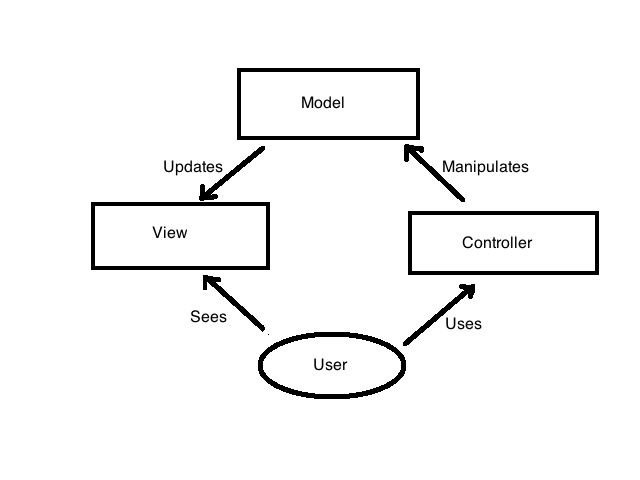
\includegraphics[width=\textwidth]{MVC.png}
                            \caption{MVC (Model View Controller) pattern}
                        \end{figure}
                        On this figure we see how user actively participates to the rendering of the website. Moreover, on this figure, Model
                        can be located server-side, so that one user action performs an update of all other users' view (example: chatting or mailing sites).\\


                        \begin{figure}[H]
                            \centering
                            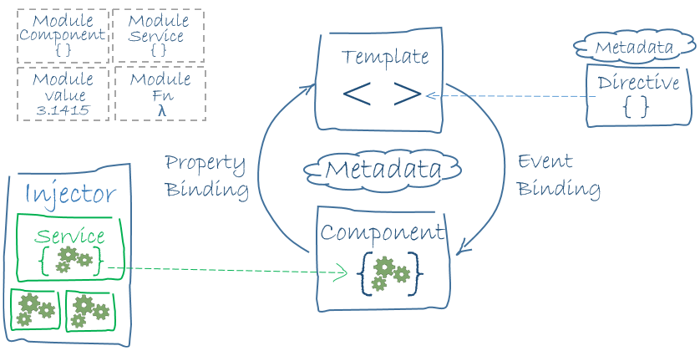
\includegraphics[width=\textwidth]{overview.png}
                            \caption{Overview of an Angular basic pieces relations}
                        \end{figure}
                        ``Together, a component and template define an Angular view.
                        A decorator on a component class adds the metadata, including a pointer to the associated template.
                        Directives and binding markup in a component's template modify views based on program data and logic.
                        The dependency injector provides services to a component, such as the router service that lets you define navigation among views.''
                        (from \href{https://angular.io/guide/architecture}{documentation})


                        There is still some similarities between websites and mobile applications.

                \subsection{Developing mobile applications}
                    As the web, mobile applications sector has hugely grown \cite{grown} since the first iPhone release in 2007 \cite{iphone}.
                    Mobile applications became more and more numerous and complex, following the global growth of smartphones perfomances:
                    processors, screens quality, storage, networks (4G). Some applications are pre-installed softwares (mail services, calculator...),
                    other ones can be found on online stores (Google Play Store, App Store).

                    \subsubsection{Basic approach}
                        One way to create mobile apps is to develop natively. Native mobile applications' strenght is that developers use 
                        built-in environment, which is adapted to each type of device. However, native applications are costly. Indeed, you need
                        to develop the same application for each operating system. 
                        \begin{table}[H]
                            \centering
                            \caption{Require skill sets for some OSes}
                            \begin{tabular}{|l|l|}
                                \hline
                                \textbf{Mobile OS type} & \textbf{Skill set require} \\ \hline
                                Apple iOS               & C, Objective C             \\ \hline
                                Google Android          & Java (Harmony)             \\ \hline
                                BlackBerry              & Java (J2ME)                \\ \hline
                                Windows Mobile          & .NET                       \\ \hline
                            \end{tabular}
                        \end{table}
                        Moreover, native developers are experts and they can work in
                        only restricted domain, focusing on single operating system. 
                        
                        One other way develop mobile apps is to use frameworks to make hybrid applications.

                    \subsubsection{Hybrid application}
                        In the same way as website development, the use of frameworks can be interesting for some companies needs or ressources.
                        An hybrid app is an app created in one single project, and available for several platforms.
                        Developing hybrid apps has several advantages: one project generates an application for several platforms, so you 
                        are sure of the integrity of the application across platforms. Moreover, maintaining is easier as developers are no longer
                        experts in a restricted area.

                        However, cross-platform apps have the disadvantage to be less performant than native ones.

                        \textbf{Ionic Framework}\\
                        Ionic Framework is a very famous mobile app framework. It is written is Angular (JavaScript) and HTML. It provides
                        built-in UI Components, API, Icons, theming, which simplifies the app developing. Ionic apps are actually websites
                        running on device browser, which access basic functionnalities of the device using Cordova.
                        That's why the cons of Ionic Framework is that applications are quite heavy, and depending on the device power,
                        application can look slow.\\

                        \textbf{React Native Framework}\\
                        \href{https://facebook.github.io/react-native/}{React Native framework} was developed by Facebook company. 
                        It is written in JavaScript. It also provides built-in components. Its strenght is that it builds native
                        mobile apps using JavaScript and React.



                    
                    \subsubsection{Web applications}
                        Web applications are quite different from mobile applications. They are actually programs that the user runs
                        in a web browser \cite{webapp}. They have the advantage to be accessed from everywhere without an app installed
                        on the device. Usually most of desktop web-apps have a reponsive design and then are accessible on smartphones
                        or tablets.\\
                        Sometimes web applications can even be better than mobile applications. In this \href{https://medium.com/@addyosmani/a-tinder-progressive-web-app-performance-case-study-78919d98ece0}{case study},
                        we can see how Tinder, a meeting app, has substancially increased both their performance and their user experience
                        using React framework to develop their webapp.

                \subsection{Use of external APIs}
                    Big companies such as Facebook, Instagram, or Google Maps, propose to developers some ways to use their data, with public
                    APIs. This allows developers to benefit huge databases and services.\\
                    For websites, public APIs come most of the time as a package.
                    In term of mapping, there are several solutions, like Bing Maps, Leaflet, but the most popular one is Google Maps. It is actually the most
                    popular API on the Internet (www.programmableweb.com/apis).


        \newpage
        \section{Objectives}
            \vspace{1cm}
            The main objective of this thesis project was to get familiar with web and mobile front-end
            development tools and technologies, but also with Google Maps API, so that I could be able to develop a new geolocation feature both on a 
            website and on a mobile application. \newline


            The second objective was to continuously investigate the web and mobile projects to focus
            on several improvements : the most important being performance improvement, but also on user experience
            improvement.
            
            \vspace{1cm}

            I worked on this thesis project in parallel of an internship in a French startup. To make
            my work more understandable, I will talk about the context of this project in the next section.


        \newpage
        \section{Context}
            This part will give a highlight about my work context. My thesis project is being developed in
            parallel with my internship in xendera, a French startup. First I will give a brief presentation
            of the company, and then I will talk about its products.
            \subsection{Xendera company}
                "xendera" is a start-up created in 2015 and based in Biarritz (France). Xendera
                is a mobile application, available on iOS and Android, encouraging participation in sport
                with discount vouchers or presents for every achieved goal.
                \newline
                Xendera's CEO and founder is Andy Guggenheimer. Xendera is his fourth company, the
                others being :
                \begin{itemize}
                    \item{AgSport Consulting, a consulting company in sport}
                    \item{Mub, a sport and travel bags company}
                    \item{MyMoneyTime, the first version of the mobile application}
                \end{itemize}
                Xendera came out on the stores in April 2017. It is the "2.0" version of the previous
                application MyMoneyTime, which had the same vocation: rewarding its users' efforts.
                Xendera offers both a graphical, functional and technological redesign.
                \newline
                Xendera is a startup: there are 22 employees, including 4 interns and 6 remote ukrainians developers. Revenues are raised
                from partnerships and investors (more than one million euros raised since 2017).
                This application has today more than 100 000 users.
                \newline
                There is three teams :
                \begin{itemize}
                    \item{marketing team (finding of partnerships, advertising, integrity of the mobile app, community managment)}
                    \item{sales team (sale of BtoB solutions, finding of partnerships)}
                    \item{IT team (developing of mobile app, back-office website, API)}
                \end{itemize}
                I worked within the IT team, that includes one CTO, two backend developers, five mobile developers,
                one DevOps and four interns.
                \newline
                This period is quite important for the company. A new mobile application (dedicated to BtoB partners)
                had to be developed, a graphical and perfomance-focused redesign of the back-office platform was planned,
                and new major features on existing mobile application had to be developed.
                
            \subsection{Xendera mobile application}

                \textbf{App use} \newline
                Xendera application make the link between users activities,
                registered via tracking application (Strava, Garmin, Runtastic...), and our database.
                Every activity from these tracking applications are imported in the application. 
                For every activity, users are given a certain amount of
                points, according to the time they run, the number of steps they made during the day, etc.
                With these points they can unlock vouchers to benefit some discounts in our partners shops or on their
                website. Users can also subscribe to challenges where they have some objective to achieve in
                order to win some presents.

                \textbf{App technologies} \newline
                Xendera BtoC mobile application looks the same on iOS and Android, however, these two applications
                are actually two distincts projects :
                \begin{itemize}
                    \item{iOS native application, developed in Objective C}
                    \item{Android application, developed with Ionic Framework}
                \end{itemize}
                Xendera BtoB mobile application is an application the mobile team developed during my internship. 
                It is the same as BtoC with company linked features, as collaborative challenges. It is written
                in React Native, a framework created by Facebook company. It generates cross-platforms
                (both for iOS and Android) native applications . The purpose of this new native and cross-platform application in the future 
                is to replace BtoC application, to improve its performance and integrity between platforms.

            \subsection{Xendera API and infrastructure}
                xendera API is composed of a MongoDB database, and services written in Scala programming language.
                API runs on nginx web server, using Docker Swarm. API main services are login, activity imports,
                HTTP requests on database objects, aggregations (statistics).
            

            \subsection{Backoffice platform}
                Backoffice platform is a website which is used to create challenges, vouchers, brands.
                It is dedicated to xendera's employees, and it is also a platform that the company proposes 
                to BtoB clients, in order to create content dedicated to employees. It is written with Angular 
                framework, a web framework using TypeScript language and developed by Google.
            
            \subsection{Xendera web application}
                One objective of the company is to propose a web application to users, so that they can manage
                their account, unlock vouchers or subscribe to challenges, directly from their computer. This
                web application will be developed with React framework.
        \newpage
        \section{Methods}
            \subsection{Specifications}
                For most of the products the company develop, a first version of the specifications
                was written by the CTO, after discussion with sales team. Then a first version
                of road map is written, and updated along the development of the product.
                Most of the features we develop and bugs we resolve are directly pointed out by
                users experience and/or requests.

            \subsection{Work environment}
                Each of the developers use Visual Studio Code, a lighter version of Visual Studio,
                as an IDE. It includes support for Git, syntax highlight, code 
                formatting and completion, and extensions can be installed.\newline
                We also use Postman to raw API use, and Studio3T for database manipulation. 

                \textbf{Jira} \newline
                We use Jira management software. Specifications are written as tasks, subtasks,
                each of them having a notion of priority, and being assigned to a developer. \newline

                \textbf{Git} \newline
                We also use the very popular Git control system. It allows several people to work
                on the same project and to keep all the project's history. GitLab is used as a Git-repository
                online manager, that provides wiki, issue tracking and continuous integration pipelines.\\
                Each developer works on a Git branch which corresponds to one Jira task.\\
                
                
                There is one environment
                dedicated to pre-production : database, website, application, API, and another one dedicated to production.
                Pre-production environment is dedicated to internal continuous testing and verification before the official release date.


            \subsection{Kanban method}
                As said previously, we used Jira as a management software. Jira provides support for Kanban methodology,
                with customable boards. It allows a better understanding of work and workflow \cite{kanban}.
                There is a total transparency for the team members.
                \begin{figure}[H]
                    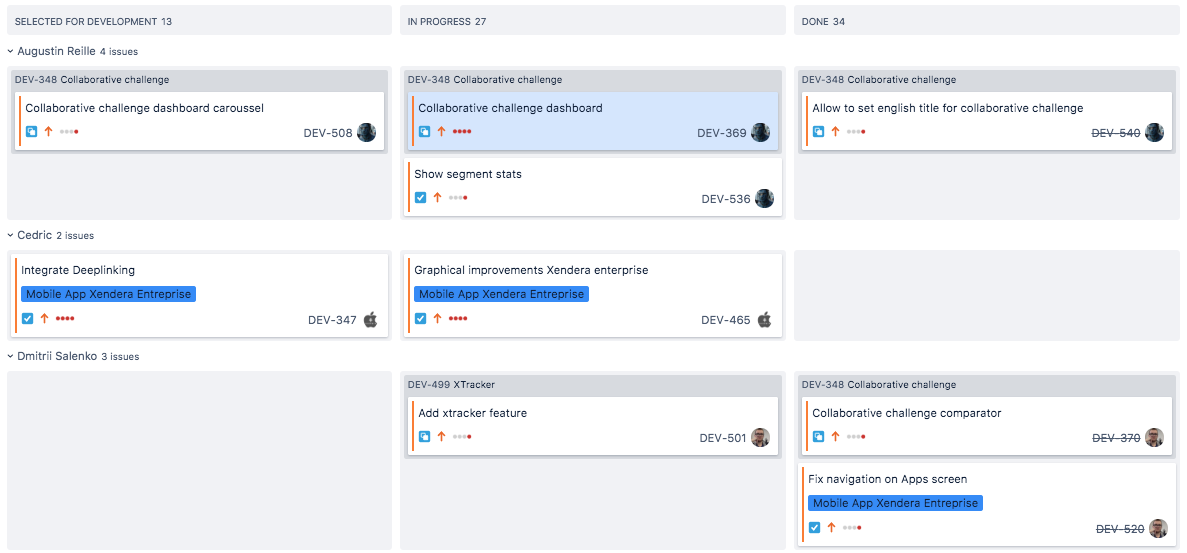
\includegraphics[width=\textwidth]{kanban.png}
                    \caption{Screenshot of our Kanban board on Jira website}
                    \label{fig:kanban}
                \end{figure}
                Every specification or bug report induce the creation of a ticket. This ticket goes in a list called "Backlog".
                At the weekly meeting at the start of the week, Backlog tickets are assigned to developers as a work for the week.
                Assigned tickets are called "Selected for Development" and go in the relative column (see fig. \ref{fig:kanban}).\\
                Every morning, a standup meeting takes place in order for each develop to talk about its work progress and its work plans for the day.
                Each developer is responsible for his task (ie his tickets) and choose the order in which he wants to do his tickets
                (taking into account the ticket priority, symbolized by colored arrows in fig. \ref{fig:kanban}).
                Placing a ticket in "In Progress" column must be done in parallel with the creation of a merge request on GitLab,
                with a "WIP" prefix so that other developers can see the code at the end of the task (see below).
            \subsection{Task implementation}
                In order to close a task, we obvioulsy have to code the expected feature or bug fix outlined in the description.\\
                Coding steps can differ according to the technology used and/or the character of the task (feature or bug).
                However there are redundant steps.\\ For new features developing (with Angular language):
                \begin{itemize}
                    \item{take in hand API routes related to the feature using Postman}
                    \item{writing of service file (link between the API and the rest of code)}
                    \item{writing of component file (API data treating)}
                    \item{writing of template file (link between the code and the user view) and styling}
                    \item{local testing (see below)}
                \end{itemize}
                For bug fixing, it depends on several things and the resolution time can be quite long: is the bug localized or not,
                is the bug resolution breaking other functionalities, etc.
            \subsection{Code review and testing}
                As mentioned earlier, GitLab website provides CI pipelines, which are run at each Git push action. At the moment,
                pipelines only build the project on a Docker container (same as production servers). One future project is to
                write tests, unfortunately we needed to upgrade to Angular v6 before doing this (more informations below).\\
                When the task is done, developer removes "WIP" prefix on the associated merge request on GitLab. Code review is assigned
                to another member of the team, which has the responsibility to validate the merge request or not. If the merge request
                is validated, the new feature or fix is deployed into pre-prodution.\\
                For mobile applications, every member of the company is invited to download the pre-production version, to use it and to share
                all its remarks. For Android app, an APK (Android Application Package) is build with the pre-production code, and is published on the Google Play
                Store as a beta-test. Beta-testers can update their application and make remarks about it. Beta-test usually lasts one week
                before release publishing.

            \subsection{Validation and deployment}
                First step of validation as a code review and testing was explained previously. Jira ticket associated to validated task can be
                moved to "Done" column of fig. \ref{fig:kanban}.\\
                The second step of validation takes into account all the other members of the company's remarks. Often, the brand manager
                or the designers have some opinions or ideas which question our work. They have access to pre-production websites or applications
                using some dedicated devices.\\
                When new features on the backoffice are validated by everyone, pre-production Git branch is merged on production branch
                and the new project is deployed.\\
                For the Android mobile app, an APK (Android Application Package) is created and posted on the Google Play Store. For iOS,
                an app file is published on Apple Store, after Apple review and validation.

        \newpage
        \section{Results}

            In this section I will talk about the results I obtained in the last months. Obviously I will only present 
            the functionnalities I worked on. I will only talk about the one major feature (which is geolocation support implementation) I developed 
            and will skip bug fixing or minor features development, for the sake of relevance.

            The idea was to add a location to our partners' stores in
            order to implement an "Around me" map on the mobile application, so that the users can see which discounts are
            accessible near them. Each of our partners have an associated Brand (which is a database object containing relative informations).
            We decided to use Google Maps APIs to implement this.\\

            First step (done by back-end developers) was to add a location support for the database brand model, then to update the API.
            The second step purpose was to add a back-office support for adding, removing, editing a brand geolocation.

            \subsection{Backoffice platform}
                The component I developed is used in the brand creation/edit page. It is accessible from a datatable listing all the brands.

                \subsubsection{Adding Google Maps API support} \label{support}
                    First step to use Google Maps API was to ask an API key. This key allows Google Maps to measure the use of their API. 
                    If the use becames too important, some pricing solutions are proposed. 
                    Google Maps API is a JavaScript API. That means that you have to load it as a script in your main HTML file:
                    \begin{lstlisting}[language=HTML]
    <script src="https://maps.googleapis.com/maps/api/js?key=YOUR_API_KEY&callback=initMap" async defer></script>
                    \end{lstlisting}
                    For Angular project, you also have to install Google Maps types for typescript support:
                    \begin{lstlisting}[language=bash]
    npm install — save @types/googlemaps
                    \end{lstlisting}
                    And import these types into our component
                    \begin{lstlisting}[language=bash]
    import { } from ‘@types/googlemaps’;
                    \end{lstlisting}
                    
                    Last step is to create an HTML div and bind it to our component, so that it can be turned into a Google Map JavaScript object.
                    This is from \href{https://developers.google.com/maps/documentation/javascript/tutorial}{documentation} the way to do it in vanilla
                    JavaScript:
                    \begin{lstlisting}[language=html]
    <div id="map"></div>
    <script>
      var map;
      function initMap() {
        map = new google.maps.Map(document.getElementById('map'), {
          center: {lat: -34.397, lng: 150.644},
          zoom: 8
        });
      }
    </script>
                    \end{lstlisting}
                    
                    
                \subsubsection{Component operation}
                    \textbf{On initialization}\\
                    Angular provides a callback method called \texttt{ngOnInit()} that allow the developer to add some others initialization
                    tasks to the component. In this method the component needs to:
                    \begin{itemize}
                        \item{create a map object and assign it some place in the HTML template}
                        \item{check if brand has a locations field}
                        \item{display map and already existing brand locations}
                        \item{get the brand address(es) from coordinates}
                        \item{display the brand address(es)}
                    \end{itemize}
                    \begin{figure}[H]
                        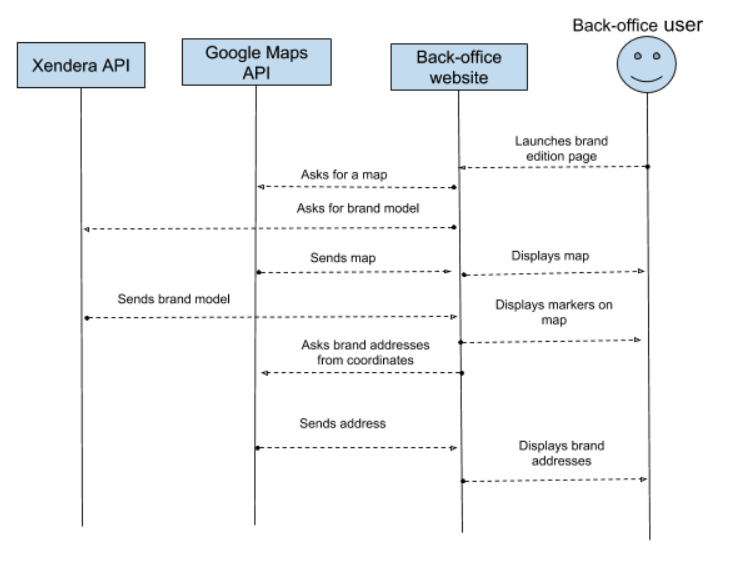
\includegraphics[width=\textwidth]{init.png}
                        \caption{Flowchart representing initialization of geolocation component}
                    \end{figure}
                    This flowchart resumes the previously listed tasks which happens in the initialization method, whith the differents actors.\\
                    
                    \textbf{On use}\\
                    For adding an address, user should be able to:
                    \begin{itemize}
                        \item{type an address}
                        \item{see this address corresponding coordinates on a map}
                        \item{validate or refuse the address}
                    \end{itemize}
                    \begin{figure}[H]
                        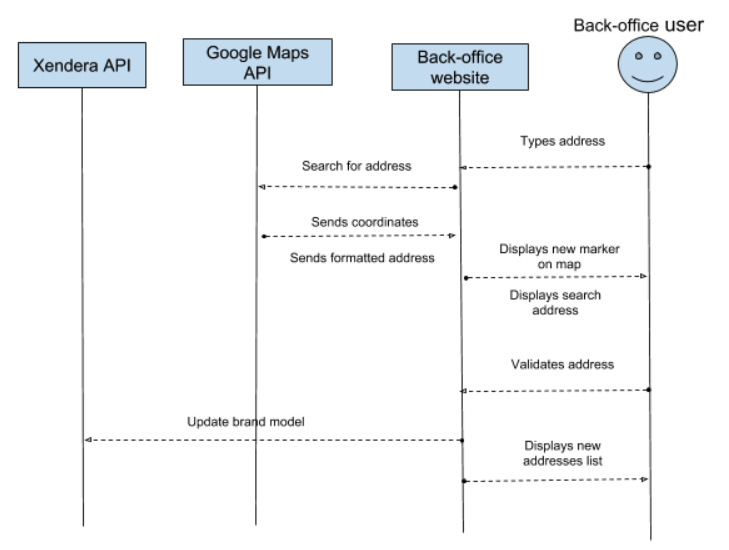
\includegraphics[width=\textwidth]{use.png}
                        \caption{Flowchart representing use of geolocation component}
                    \end{figure}
                    This flowchart resumes the previously listed tasks which happens in the use of component, whith the differents actors.\\

                \subsubsection{User interface implementation}
                    \begin{figure}[H]
                        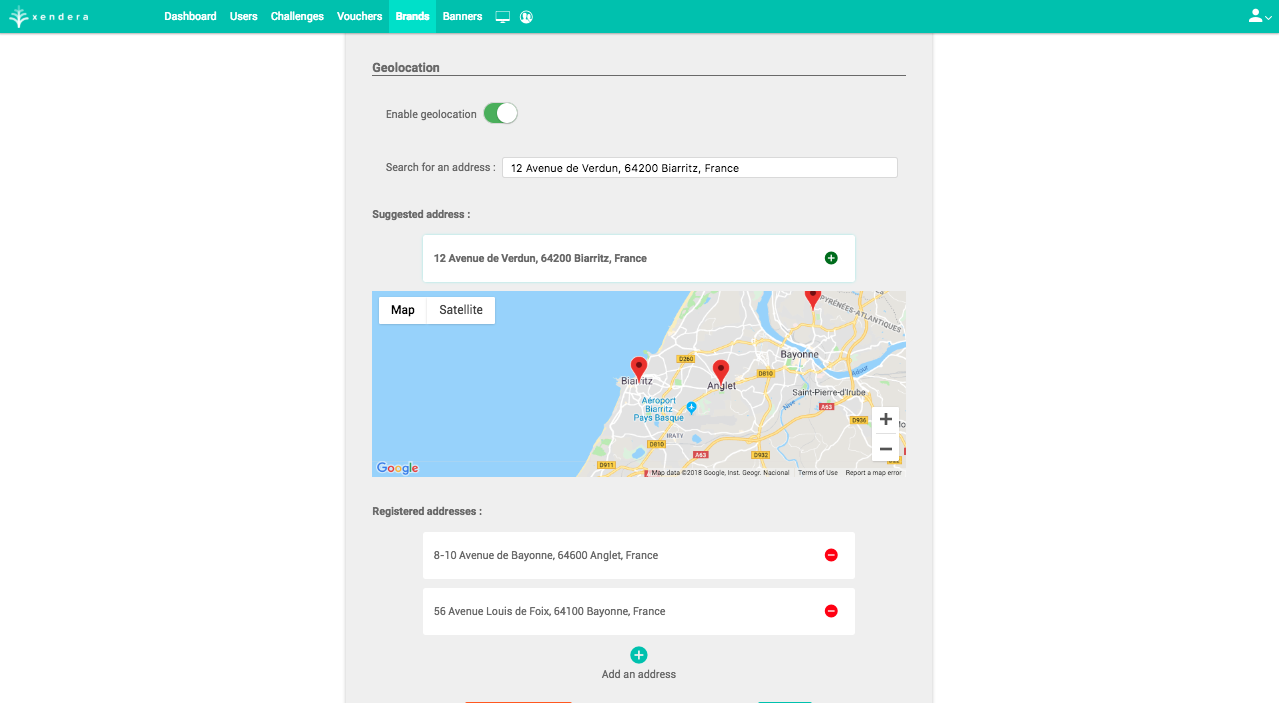
\includegraphics[width=\textwidth]{geolocation_web.png}
                        \caption{Screenshot of geolocation component on back-office website}
                    \end{figure}
                    Back-office user can type an address in an HTML input, which will be searched using Google Maps API, and display on a map (also provided
                    by Google Maps API). Actually, address is converted in a location using latitude and longitude coordinates.
                    Location can be added to the brand model using the "+" button. User is notified using a toaster on the 
                    top-right corner of the website everytime something happens which is not visible (successful or failed update, network or login error...).
                    A security also forbids the entering of an already-registered location.\\
                    Initially, only one address could be selected. However, we signed a contract with MacDonald's, and they were going to provide
                    vouchers availables in fifty restaurants. We decided then to implement a multi-location logic.
                    
            \subsection{xendera Android mobile application}
                Third and last development step for global geolocation feature was to implement an "Around me" page in the app.\\
                \textbf{NB: } As the Android mobile application also uses Angular, the Google Maps API integration in project is the same. Please see \ref{support}.
                
                    \begin{figure}[H]
                        \centering
                        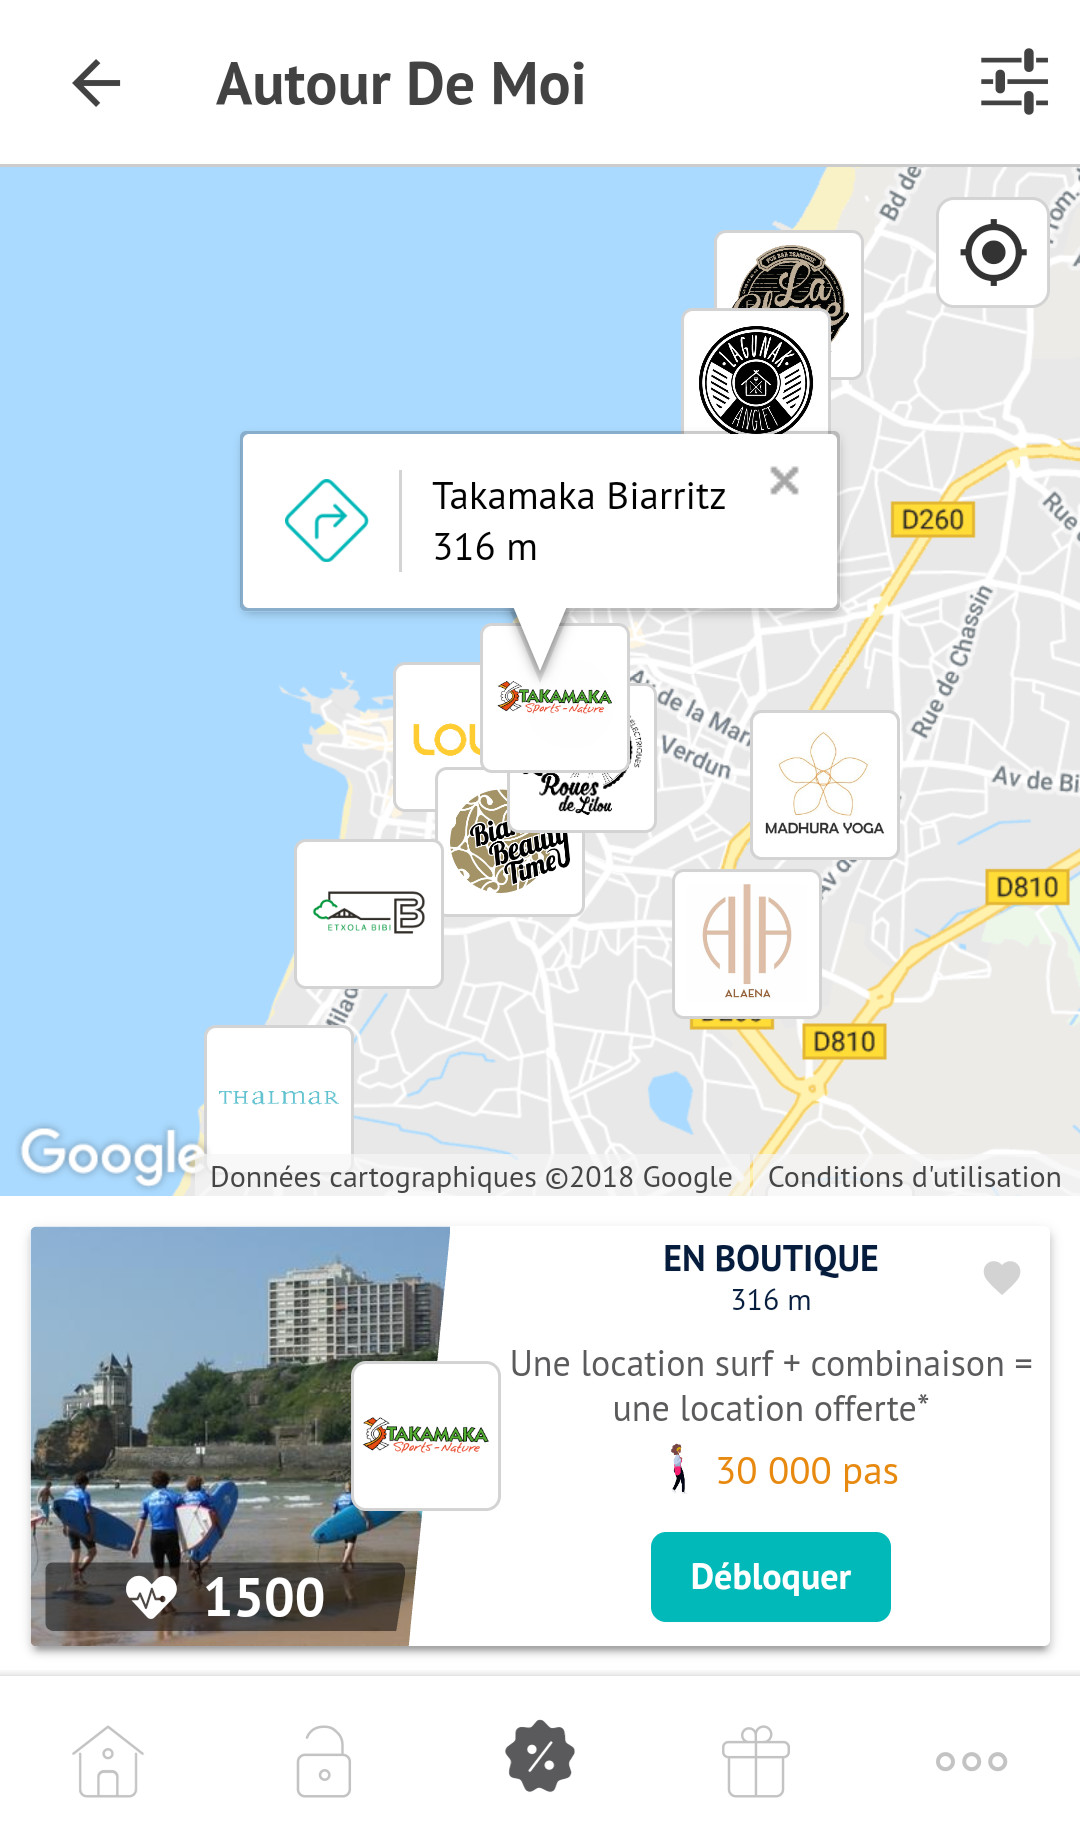
\includegraphics[width=6cm]{geolocation_app.jpg}
                        \caption{Screenshot of geolocation page on Android mobile app}
                        \label{fig:app}
                    \end{figure}

                    On this page, user can see shops (and associated vouchers) located near him. There is a filter option (each brand has categories) on
                    header's top right, a recenter button on map's top right. Brand logos are customed Google Maps objects I had to develop. Hopefully Google Maps
                    API let developers the possibility to customize its ressources.
                    When user clicks on a brand logo, associated vouchers appear on the bottom page, and a marker reminds the brand name and the distance to the store.
                    When user clicks on a marker (which is also a custom Google Maps marker I had to develop), it open a navigation application (like Google Maps,
                    Apple Maps or Waze).
                
                \subsubsection{Displaying map and brands locations}
                    First step was to display a map on the application page, and to display API's brands locations. Basically every brand has the following model:
                    \begin{lstlisting}
    {
        "uuid": "db0738e2-0e8b-4aab-96a2-c9909902afba",
        "createDate": "2017-11-15T09:44:02+00:00",
        "updateDate": "2018-06-18T20:37:36+00:00",
        "name": "Lyon Cycle Chic",
        "logoPictureUrl": "https://api.xendera.io/v1/assets/d636e4aa-7eda-411b-a728-7e814576baad",
        "locations": [
            {
                "lng": 4.8441098,
                "lat": 45.7495649
            }
        ]
    }
                    \end{lstlisting}
                    I needed to create a Google Maps Marker on each brand location which should be displayed on the map. When clicking on the marker,
                    vouchers associated to the brand must be shown as on Figure \ref{fig:app}. This voucher was an already existing component, which was
                    used on the vouchers list on the application. I only had to reuse it in my page.

                \subsubsection{Creating custom Google Maps components}
                    Second step was to improve the brand display design, as on Figure \ref{fig:app}, with brands logos inside some squares. Google Maps API
                    provides some documentation to make custom components but it is written in JavaScript, so I had to translate it into TypeScript.\\
                    An other feature we wanted to implement was the navigation tool : by clicking on the info window above selected brand, a pop up should
                    let the user select which navigation app he wants to use to get to the brand address. I also had to develop this custom Google Maps InfoWindow.

                \subsubsection{Use of external tools}
                    Some external tools allow the application to get informations on the device.
                    For this page I used several external tools. One of the most important was a tool which let the application know if the user has activated
                    the location services on his device. Indeed, we could not get user's position if the location services are shut down.
                    \\
                    The other package I used is a package that allows Ionic applications to list all navigations applications present on the device and let 
                    the user choose which one he wants to use to go to an input position or address.
                    
                    % \begin{figure}[H]
                    %     \centering
                    %     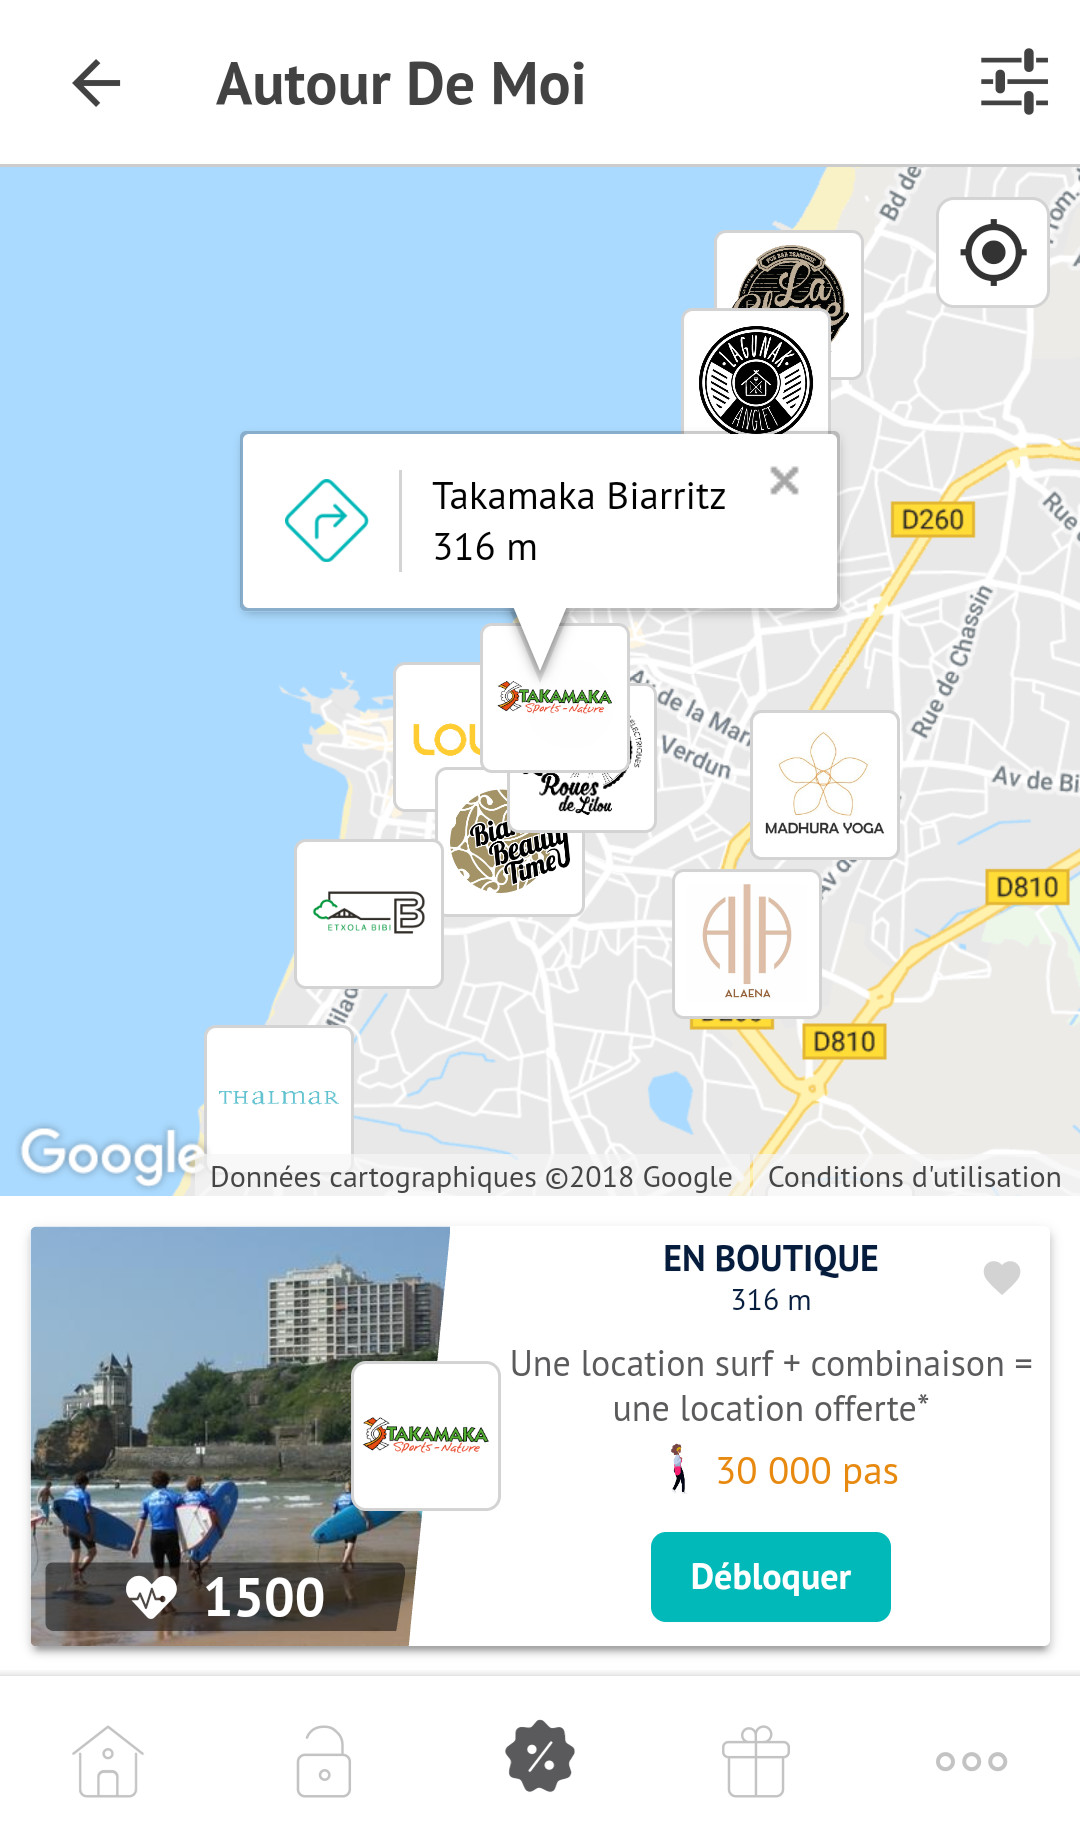
\includegraphics[width=6cm]{geolocation_app.jpg}
                    %     \caption{Screenshot of geolocation page on Android mobile app}
                    % \end{figure}
                    
        \newpage
        \section{Discussion}
            \subsection{Development process}
                As a matter of fact, I already spent a four month internship in this company last year. It was a different CTO and we were less developers in the team.
            We used Scrum methodology, which was quite efficient, however we did not use Jira tool and that is the major improvement I pointed out.
            Indeed, with the tasks system and Kanban methodology, we have a cleaner Git history and better transparency. Furthermore, we did not practice
            code review and local testing, tests were run directly on pre-production environment. Now, bugs, errors or missing features are spotted earlier
            and this is an important time saving.\\

            One strenght of Scrum I did not found in Kanban methodology is that with Scrum task notation system, the team tends to know exactly which feature can be developed in
            a certain amount of time. However, the new CTO is more experimented in project and team managment, and his estimations on delays were quite right.
            Kanban methodology and the new manager gave to the IT team more seriousness.\\

            Yet, I think this is quite difficult to make all members of a team being rigorous about development methods, mostly if previous one were less rigorous.
            
            \subsection{Geolocation feature}
                \subsubsection{Back-office website}
                    I already worked with public APIs such as Instagram API, and it was quite restrictive and not well documented. I was pleasantly suprised
                    by the quality and clearness of the Google Maps API documentation. It provided good way to customize components, and a very quick and accurate
                    API address search.
                \subsubsection{Mobile app}
                    This page was quite long to develop. Specifications for it evolved almost every day (for styles but also for features). As we 
                    worked at the same time with the mobile iOS developer, we had to adapt to each other technologies and possibilities. iOS features for
                    this page were pretty easy to implement, while it was tricky with Ionic. Also, we decided to add the navigation feature and had 
                    discussions about it, which took some time over development. Fortunately, the card at the bottom of the page was a component
                    which was already coded and I had no difficulties to use it in this page.\\

        \newpage
        \section{Conclusion}
            This thesis project was focusing on new technologies processes in the field of web and mobile front-end development. The purpose was to give and idea about
            the pertinence and the efficiency of the use of an external API (Google Maps API) to implement a geolocation feature.
            
            \vspace{1cm}

            Nowadays, more and more companies rely on bigger companies' public API to offer to their users a quality and reliable content. Moreover,
            as these bigger companies (like Facebook, Google...) are very famous and popular, users are accustomed to their use. This allows small companies
            like startups to focus on exclusive features development in a safe environment.

            \vspace{1cm}

            Moreover, the use of famous web and mobile development frameworks make their development easier, by providing components but also community-made and
            open-sources packages which can save developers a lot of time. This allows small companies to increase their competitiveness, by offering more and more
            qualitative content. However, big companies like Facebook or Instagram's supremacy is very difficult to contest and concurrencing companies like this is 
            almost impossible.

            \vspace{1cm}

            Though, with recents european laws, big firms supremacy and user's data use can be contested. It should have been interesting for example to
            use a different Map provider (for example Leaflet, which is open-source) for the features I develop, and to compare performance and user experience.
            However this is almost impossible to implement is a start-up environment.

            \vspace{1cm}
            
            These features I developed are deployed and in production since a month. We do not have enough user experience feedback to know if the
            geolocation suits them, on the other hand, this geolocation feature was something very asked and attractive for partners and it may have impacted their involvement
            in the xendera's offer.
            
            \vspace{1cm}

            My future work on this feature is still unknown, but it could change very quickly by users or client demand. As a future task, I will
            participate on the development of the future web application, which will be developed in ReactJS, another web framework, which certainly
            offers a lot of advantages, as the ones I already used.
            
        % References
        \newpage
        \section{References}
        \begin{thebibliography}{9}
            \bibitem{history}
            Cailliau, Robert. \textit{A Little History of the World Wide Web}
            \\\texttt{https://www.w3.org/History.html}

            \bibitem{compet}
            Loughlin, P. \textit{Viewpoint: e-commerce strenghtens supplier's position}, 1999

            \bibitem{presence}
            Watkin C., Marenka S. \textit{The Internet Edge in Business}, 1995 

            \bibitem{fields}
            Taylor, M.J. \textit{Methodologies and website development: a survey of practice}, 2002

            \bibitem{grown}
            Ludwig, Sean. \textit{Mobile app usage grows 35\%, TV \& web not so much}, 2012
            \\\texttt{https://venturebeat.com/2012/12/05/mobile-app-usage-tv-web-2012/}

            \bibitem{iphone}
            Cohen, Peter. \textit{Macworld Expo Keynote Live Update}, 2007
            \\\texttt{https://www.macworld.com/article/1054764/macworld-expo/liveupdate.html}

            \bibitem{webapp}
            Alex Chaffee. \textit{What is a web application (or "webapp")?}, 2012
            \\\texttt{http://www.jguru.com/faq/view.jsp?EID=129328}

            \bibitem{kanban}
            Karl Scotland. \textit{Aspects of Kanban}, 2010
            \\\textit{http://www.methodsandtools.com/archive/archive.php?id=104}

        \end{thebibliography}
    \end{document}